%!TEX root = ../article.tex

% A new section
\section{Evaluation}
\label{sec:evaluation}


\subsection{GD capability}
The goal of our work was to bring \gls{gd} to the web browser so it can be used anywhere more easily.
To do this, we implemented a set of primitives that produce several 3D concepts to be used as building blocks for modeling.

Now comes the time to test Luna Moth's ability to be used for \gls{gd}, more specifically to produce diverse 3D models.
In order to evaluate this, we developed several programs that reproduce examples that were previously done in other \gls{gd} environments.
The results of these programs are shown in Figure~\ref{fig:all:examples}.

\begin{figure}
  \centering
  \begin{subfigure}[t]{0.3\linewidth}
    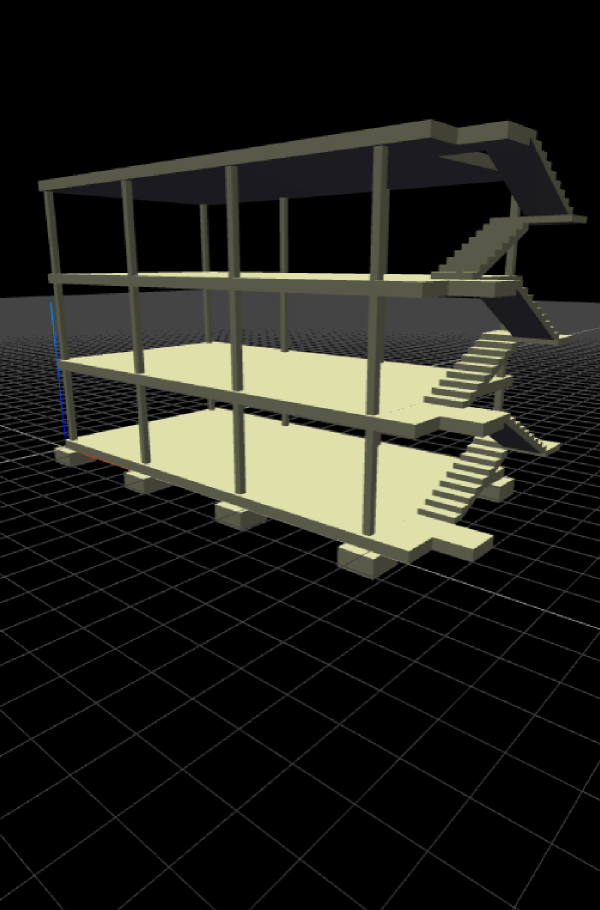
\includegraphics[width=1.0\linewidth]{./\figurePath/all_examples/dom_ino_crop}
    \caption{Dom-ino}
    \label{fig:ex:domino}
  \end{subfigure}
  \begin{subfigure}[t]{0.3\linewidth}
    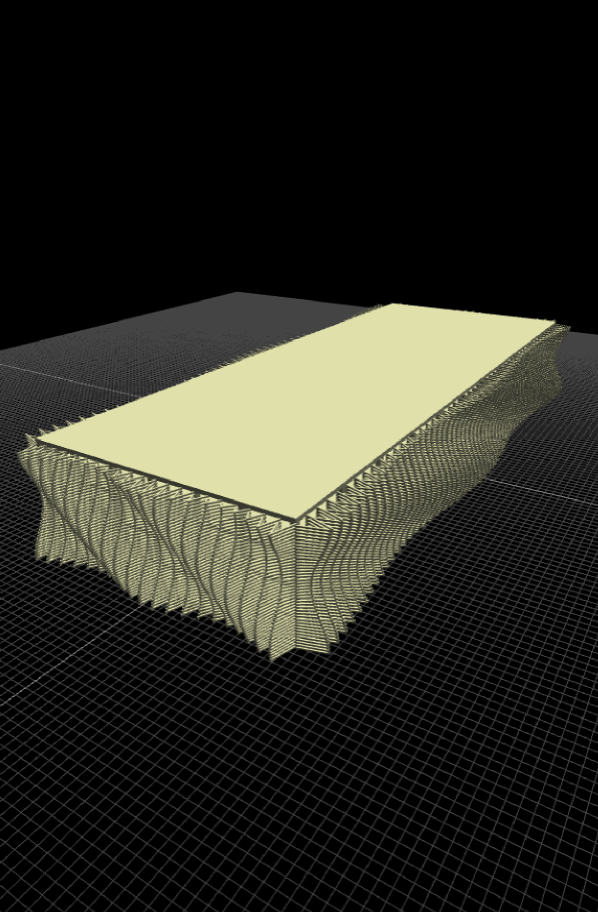
\includegraphics[width=1.0\linewidth]{./\figurePath/all_examples/edificio_carmo_crop}
    \caption{Carmo Facade}
    \label{fig:ex:carmo:facade}
  \end{subfigure}
  \begin{subfigure}[t]{0.3\linewidth}
    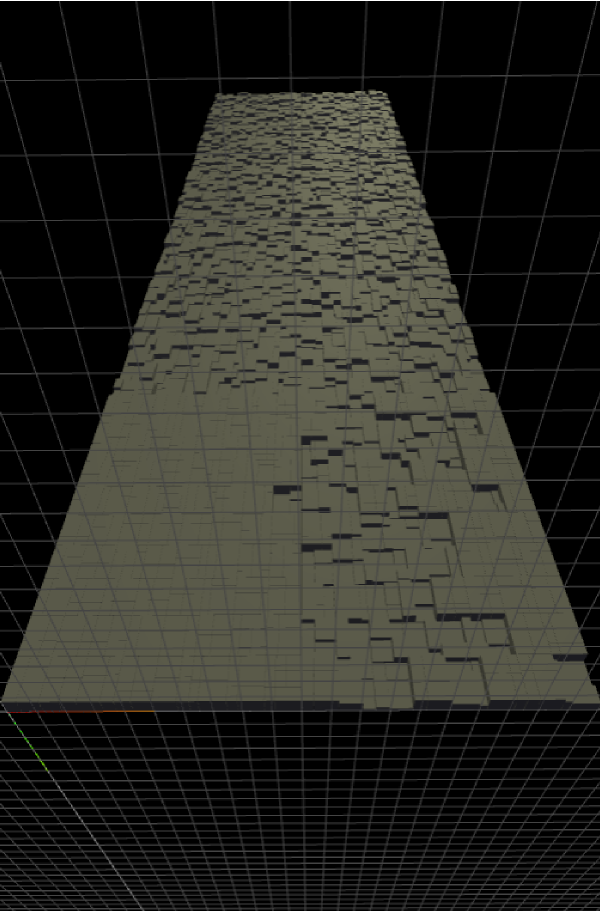
\includegraphics[width=1.0\linewidth]{./\figurePath/all_examples/sheung_wan_hotel_crop}
    \caption{Sheung-wan hotel}
    \label{fig:ex:sheung:wan}
  \end{subfigure}
  \begin{subfigure}[t]{0.3\linewidth}
    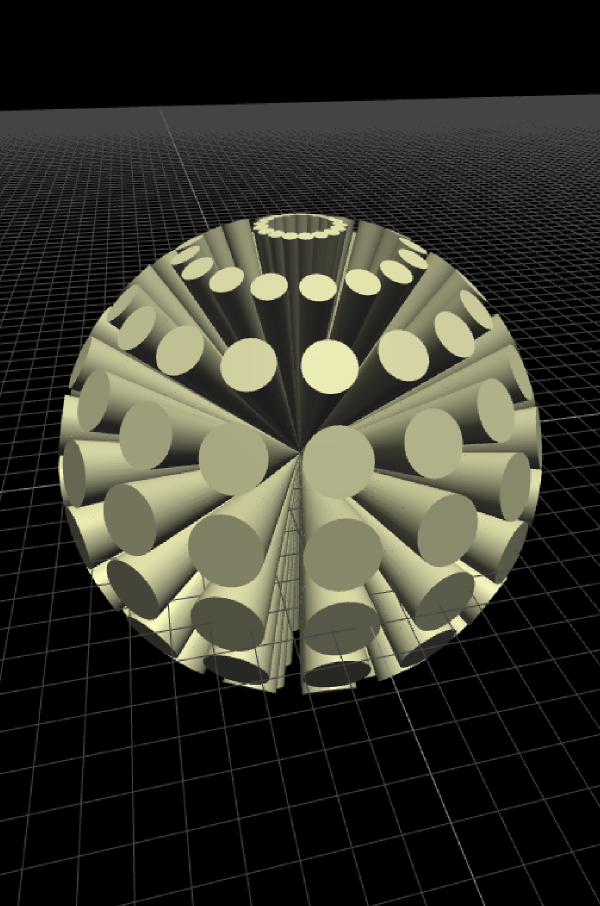
\includegraphics[width=1.0\linewidth]{./\figurePath/all_examples/coneSphere_crop}
    \caption{Sphere of cones}
    \label{fig:ex:cone:sphere}
  \end{subfigure}
  \begin{subfigure}[t]{0.3\linewidth}
    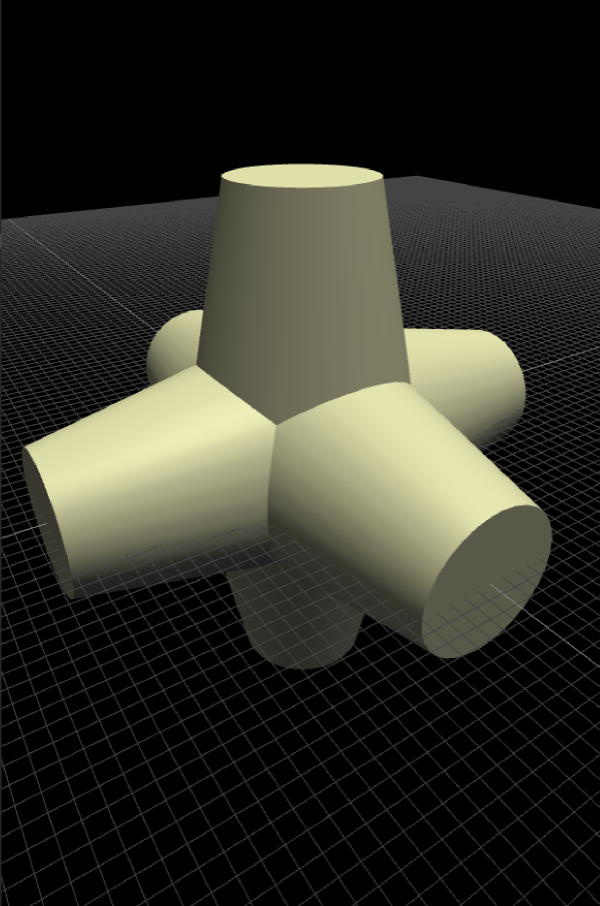
\includegraphics[width=1.0\linewidth]{./\figurePath/all_examples/ortho_cones_crop}
    \caption{Orthogonal Cones}
    \label{fig:ex:ortho:cones}
  \end{subfigure}

  \caption{Renderings of results of the implemented example programs.}
  \label{fig:all:examples}
\end{figure}

Still, the range of results is limited by the primitives currently implemented.
For example, none of these programs make use of \gls{csg} operations like union, intersection and difference as they are not implemented.
Nonetheless, it is possible to support them since there are JavaScript libraries that already implement \gls{csg}, like the case of OpenJSCAD's.
These operations should be addressed in future work.
In addition, the support for randomness and programming techniques like higher-order functions keeps the ability to create complex models.


\subsection{Performance}
We evaluated our solution's performance from different perspectives:
(1) how running performance in Luna Moth compares with other \gls{gd} environments;
(2) how running performance compares to export performance;
(3) how traceability data collection affects running performance;
(4) how export performance compares with exporting in other IDEs, like Rosetta and Grasshopper.

To make this evaluation possible, we measured times of several situations:
(1) running in Luna Moth, with traceability enabled;
(2) running in Luna Moth, with traceability disabled;
(3) exporting from Luna Moth to AutoCAD;
(4) running in Rosetta connected to AutoCAD;
(5) running in OpenJSCAD;
(6) running in Grasshopper, while generating previews in Rhinoceros;
(7) running in Grasshopper, followed by baking geometry to Rhinoceros.

The next sections presents the evaluation from the previous perspectives.

\paragraph{Setup}
All tests were performed on a Microsoft Surface Pro 4 with in Intel Core i5 processor and 4GB of RAM.
The web page and the remote CAD service were hosted at the same computer.

\begin{figure}
  \centering
  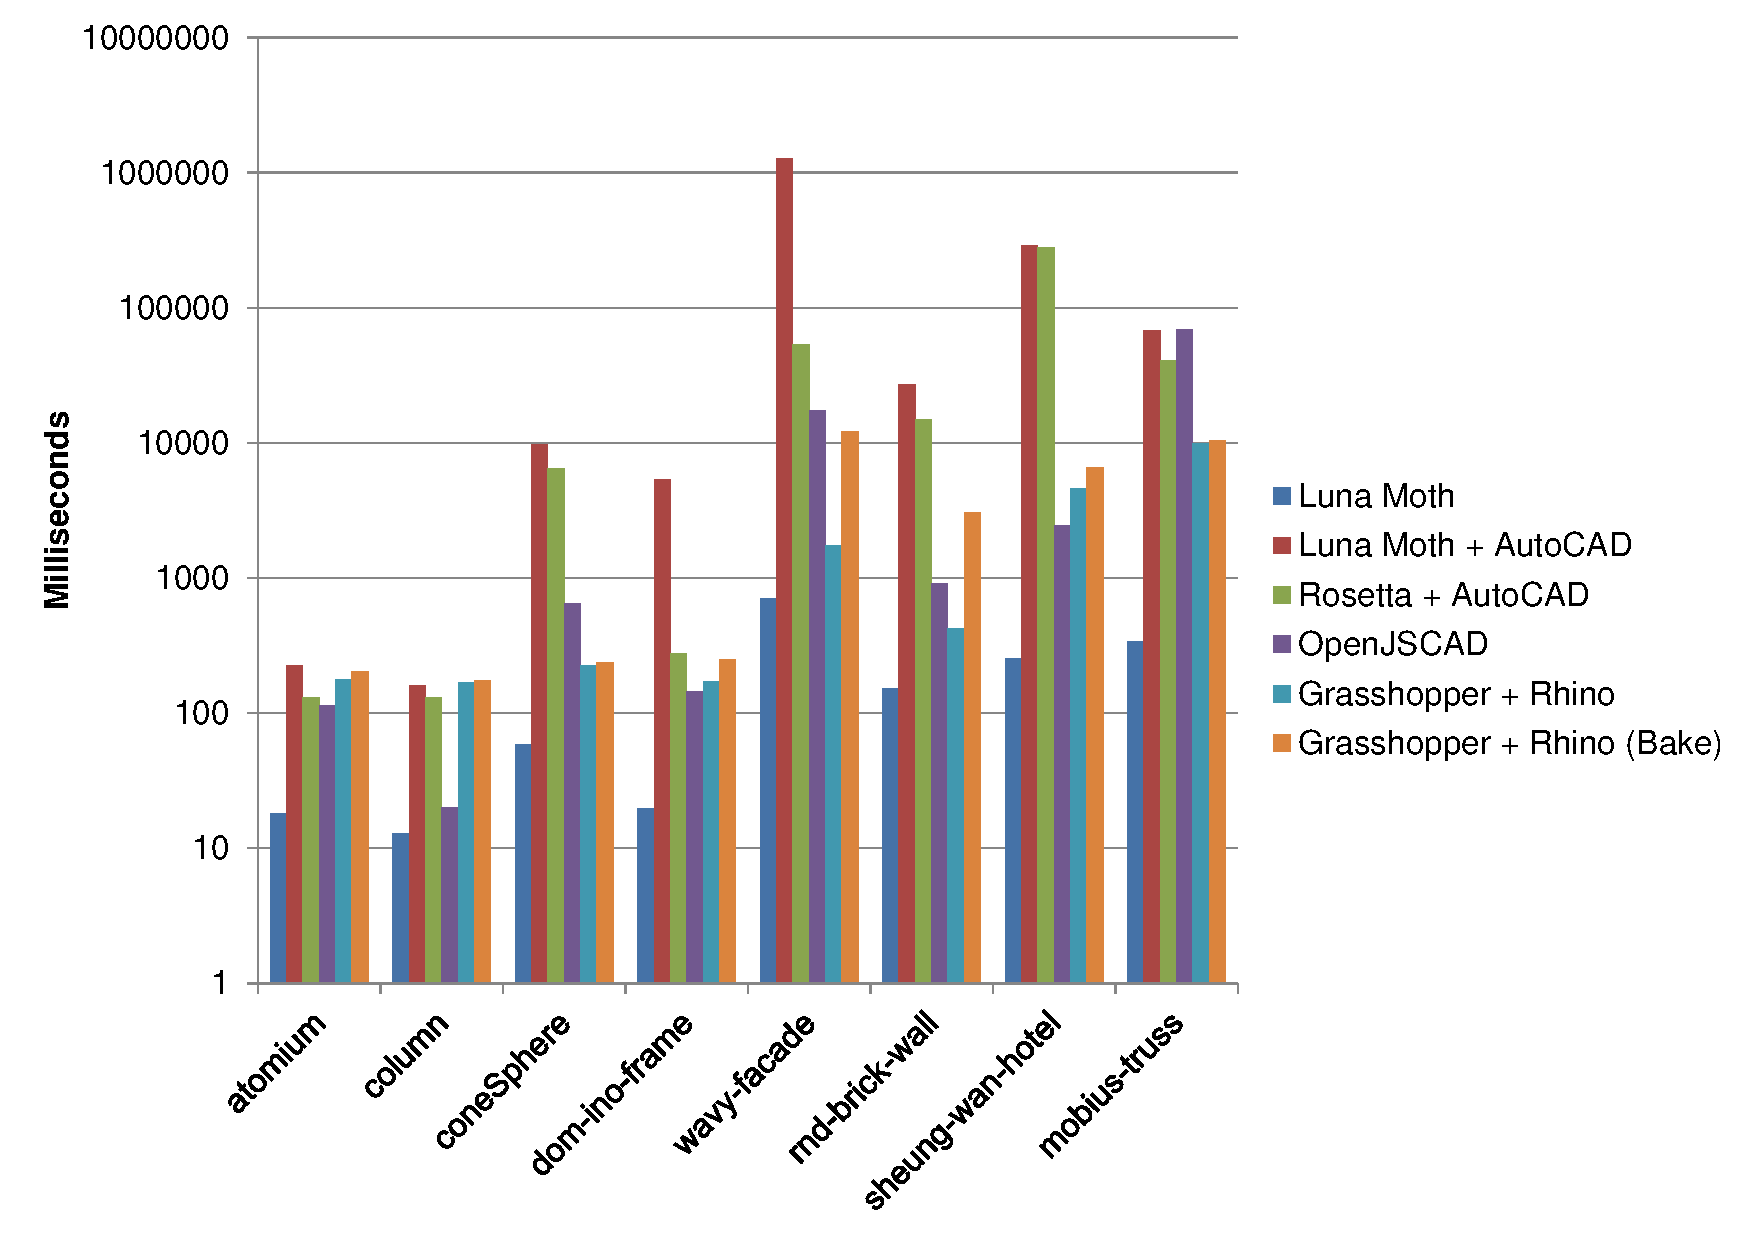
\includegraphics[width=\linewidth]{./\figurePath/run_export_rosetta_times}
  \caption[Comparison of running times for our \gls{ide}, its export process, Rosetta, OpenJSCAD, and Grasshopper.]{Comparison of running times for our \gls{ide}, its export process, Rosetta, OpenJSCAD, and Grasshopper. Note that the time is in logarithmic scale.}
  \label{fig:run:export:rosetta:chart}
\end{figure}


\subsubsection{Running Performance}
To see how the performance of our web-based \gls{gd} environment compares to the existing environments, we compared the time each takes to generate identical models.
First, we implemented a version of each program using each environment's programming language and, then, measured the time each took to complete.
These times are shown in the chart on Figure~\ref{fig:run:export:rosetta:chart}.
As can be seen, the relationship between running times varies from program to program, although Luna Moth is consistently faster than Rosetta (connected to AutoCAD), OpenJSCAD and Grasshopper (\textit{Grasshopper + Rhino}).
In some instances, we can see a difference of at least an order of magnitude.

With this in mind, we can say that our solution can provide better feedback than Rosetta.


\subsubsection{Run vs Export}
The next step was to evaluate how the execution time differs between the normal running process and the remote \gls{cad} running process.
To measure the difference, we ran the previous programs using Luna Moth's export process and measured the time each took to complete.
These times are also shown in Figure~\ref{fig:run:export:rosetta:chart}.
As seen in the chart, comparing export times (\textit{Luna Moth + AutoCAD}) to normal running times (\textit{Luna Moth}), export times range from being around twelve times to eighteen hundred times the normal running times.

Given that the difference can grow to three orders of magnitude, it is highly preferable to get feedback using the web application instead of using the export process.
The export process should be reserved to when the architect is satisfied with the obtained solution.


\subsubsection{Export vs Other IDEs}
Another comparison that we have to make is one between Luna Moth's export process and similar processes in other IDEs, namely, Rosetta and Grasshopper.
For this comparison, we took the times from our export process, Rosetta connected to AutoCAD, and Grasshopper baking geometry to Rhinoceros.%
\footnote{Grasshopper only displays previews of results in Rhinoceros while programs are being developed. To export results to Rhinoceros, Grasshopper has a feature called "Bake Geometry".}
These correspond, respectively, to \textit{Luna Moth + AutoCAD}, \textit{Rosetta + AutoCAD}, and \textit{Grasshopper + Rhino (Bake)} in Figure~\ref{fig:run:export:rosetta:chart}.
As can be seen, Luna Moth's export times range from $\approx$1x to $\approx$24x the times of running in Rosetta and range from $\approx$0.9x to $\approx$104x the times of running and baking in Grasshopper.


\subsubsection{Traceability Performance}
To measure the impact that traceability data collection has on program running time we also ran programs with data collection enabled and disabled and measured the time each took to execute.
The chart in Figure~\ref{fig:traceability:timing} shows a comparison of their times.

We can observe that running with traceability impacts the running time, increasing it by 10--50\% which, depending on the example, can be considered between a small impact and a large impact.
Like so, traceability data collection may need to be disabled to increase feedback when running complex programs.
However, the impact is worth taking when the user needs to debug the program.

\begin{figure}
  \centering
  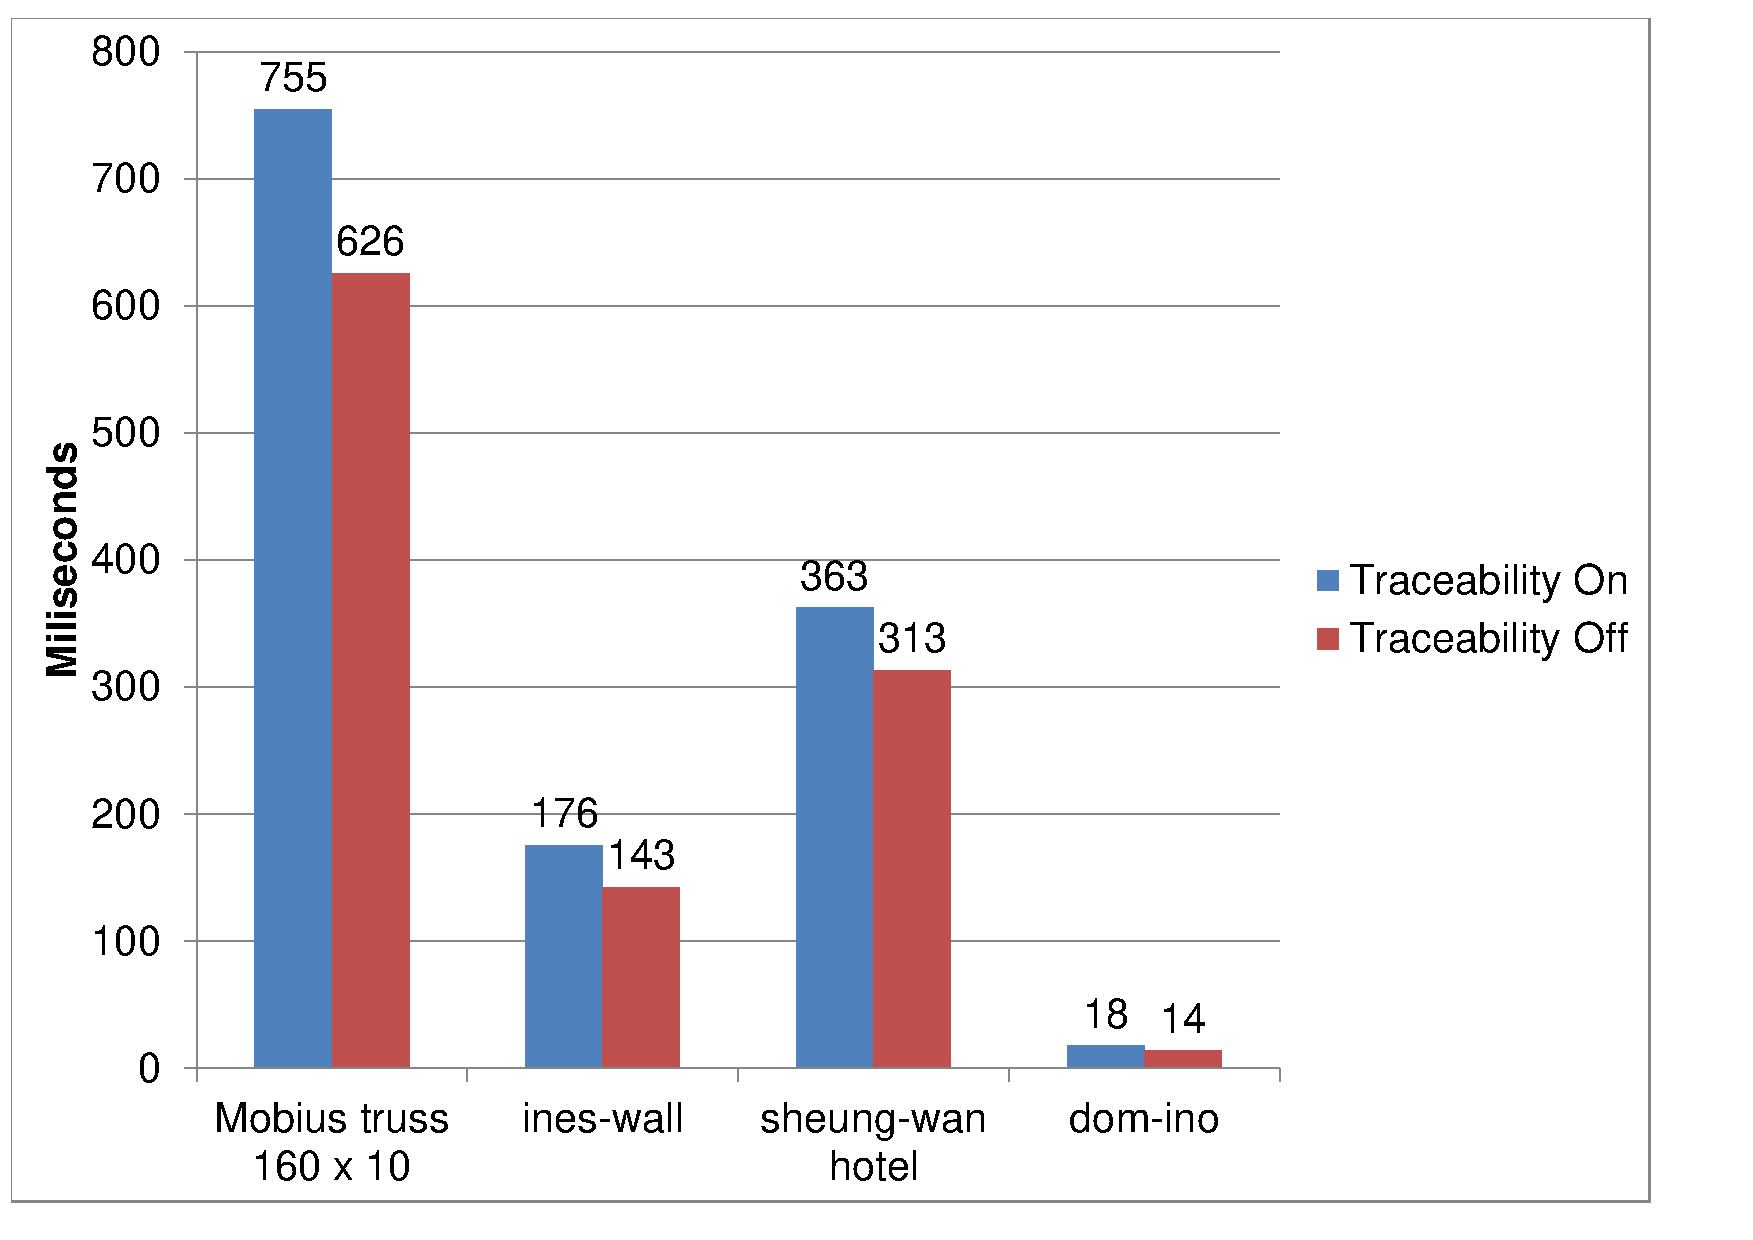
\includegraphics[width=\linewidth]{./\figurePath/traceability_timing}
  \caption{Running while collecting traceability data and while not collecting traceability data. Note that times are in logarithmic scale.}
  \label{fig:traceability:timing}
\end{figure}
